\documentclass{report}
\usepackage{blindtext}
\usepackage[utf8]{inputenc}
\usepackage{algorithm}
\usepackage[noend]{algpseudocode}
\usepackage{titlesec}
\usepackage{mathtools}
\usepackage{tikz} %% Package for drawing finite state machines in LaTEX
\usetikzlibrary{automata, positioning,arrows}
\newcommand{\me}[1]{
\begin{math}
#1
\end{math}
}
\title{Home Work 3}
\author{Francisco J. Díaz Riollano \\ Student ID: 802-15-2172 }


\begin{document}

\maketitle
 %%%%%%%%%%%%%%%%%%% First Question%%%%%%%%%%%%%%%%%%%%%%%
\paragraph{\Large{Question 1\\ \\}}


\begin{algorithm}
  \begin{algorithmic}[1]
    \Procedure{NAIVE}{\textit{On input} S[1,..m]}
      \State $n\gets |T|$
      \State $m\gets |S|$
      \For{s=0 \textbf{to} n-m}
      \If{P[1,..m] = T[s+1...s+m]}
      	\State \textbf{print}\textit{("pattern found")}
      \EndIf
      \EndFor     
    \EndProcedure
  \end{algorithmic}
\end{algorithm}


The string matching problem is defined as: "Given a text \me{T=T_1 ... T_n} which is stored as array \me{T= T[1,...,n]} , and a pattern \me{P = P_1 ... P_m = P[1...m]} with \me{m<n}, where both are strings over the same alphabet \me{\Sigma;}decide whether S is a substring of T.

Algorithm 1 is the so-called naive-pattern finding algorithm. Use Algorithm 1 to construct a Finite State. Automata(deterministic or non-deterministic) for solving the matching problem. 
\\

Let M \me{=(Q,\Sigma,\delta,q_0,F)} be 5-tuple NFSA where: \newline
Q is a finite set of states \newline
\me{\Sigma} is a finite set if input symbols \newline
\me{\delta} is a state transition function from \me{Q \times \Sigma \rightarrow Q} \newline
\me{q_0 \in Q} is the initial state \newline
\me{F \subseteq Q} Q is the set of final states \newline
Let \me{A=\{s_1,s_2,...,s_{|A|}\}} and \me{\bar{p} = A -p}.
\\
\\
High Level Description of the automata: \\
M =: "On input S[1,...,m]"

% %%%%%%%%%%%%%%%%Automata Describing the algorithm %%%%%%%%%%%%%%
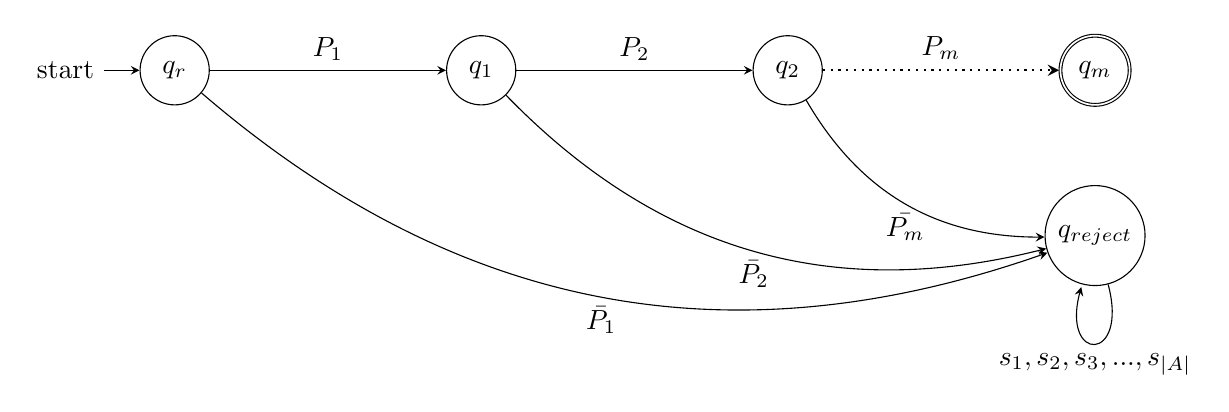
\begin{tikzpicture}[->,>=stealth] 

\node [state,initial] (q0){$q_r$};
\node[state,right = 3cm of q0](q1){$q_1$};
\node[state,right = 3cm of q1](q2){$q_2$};
\node[state,accepting, right = 3cm of q2](qm){$q_m$};
\node[state, below = 1cm of qm](qrej){$q_{reject}$};

\path (q0) edge [above] node {$P_1$} (q1);
\path(q1) edge [above] node {$P_2$}(q2);
\path(q2) edge [dotted,above,thick] node {$P_m$}(qm);

\path (q0) edge[bend right, below]  node {$ \bar{P_1}$} (qrej);
\path (q1) edge[bend right, below]  node {$\bar{P_2}$} (qrej);
\path (q2) edge[bend right, below]  node {$ \bar{P_m}$} (qrej);

%loop
\path (qrej) edge[loop below] node{$s_1,s_2,s_3,...,s_{|A|}$}(qrej);

%\path (q1) edge[bend left, above]  node {$ P_2,P_3,...P_m$} (q0);

%\path (q2) edge[bend left, above]  node {$ P_1,P_3,...,P_m$} (q0);
%\path (qm) edge[bend left, below]  node {$P_1,P_2,...,P_{m-1}$} (q0);


%\node[state,accepting](qm){$q_m$};
\end{tikzpicture}
 %%%%%%%%%%%%%%%%%%% First Question%%%%%%%%%%%%%%%%%%%%%%%%
 
 
 
 %%%%%%%%%%%%%%%%%%% Second Question%%%%%%%%%%%%%%%%%%%%%%%
 
\paragraph{\Large{Question 2\\ \\}}
Algorithm 1 returns a result in the time proportional to \me{O(|T| |S|)}. Discuss the computation time of your automaton.
\\ In the worst case the automata will have \me{O(|T| |S|)} complexity. We know this because it iterates through the whole text of size \me{|T|} and for each of those iterations it compares at \me{|S|}, which is the size of the string, individual items. Thus the automata has the same time complexity as the algorithm. 
\newline
\begin{tikzpicture}[->,>=stealth] 




\node[state,below =3cm of q0](T1) {$T_1$};

\node[state,accepting, right =1cm of T1](Acc) {$$};
\path (T1) edge[above] node{$\epsilon$}(Acc);


\node[state,right =3cm of T1](T2){$T_1$};

\node[state,accepting, right =1cm of T2](Acc) {$$};
\node [state,above=3cm of Acc](q0) {$$};
\path (T2) edge[above] node{$\epsilon$}(Acc);
\path(q0) edge [above] node {$P_1$}(T1);
\path(q0) edge [left] node {$P_2$}(T2);





\node[state,right =5cm of T2](Tn){$T_1$};
\path(q0) edge [left] node {$P_m$}(Tn);
\path (Acc) edge[above,dotted,thick] node{$$}(Tn);
\node[state,accepting, right =1cm of Tn](Acc) {$$};
\path (Tn) edge[above] node{$\epsilon$}(Acc);


\node[state, below =1.5cm of T1](2){$T_2$};
\node[state, left =0.5cm of 2](1){$T_2$};
\node[state, right =0.5cm of 2](3){$T_2$};
\path(T1) edge [left,dotted,thick] node{$T_1$}(1);
\path(T1) edge [left] node{$P_2$}(2);
\path(T1) edge [left,dotted,thick] node{$...$}(3);

\node[state, below =1.5cm of T2](2'){$T_2$};
\node[state, left =0.5cm of 2'](1){$T_2$};
\node[state, right =0.5cm of 2'](3){$T_2$};
\path(T2) edge [left,dotted,thick] node{$P_1$}(1);
\path(T2) edge [left,dotted,thick] node{$P_2$}(2');
\path(T2) edge [left,dotted,thick] node{$...$}(3);



\node[state, below =1.5cm of Tn](2'){$T_2$};
\node[state, left =0.5cm of 2'](1){$T_2$};
\node[state, right =0.5cm of 2'](3){$T_2$};
\path(Tn) edge [left,dotted,thick] node{$P_1$}(1);
\path(Tn) edge [left,dotted,thick] node{$P_2$}(2');
\path(Tn) edge [left,dotted,thick] node{$...$}(3);



\node[state,below = 3 cm of 2](f){$T_n$};
\path(2) edge[left,dotted,thick] node{$P_m$}(f);
\node[state,accepting,right = 1.5cm of f] (final){$$};
\path(f) edge[above] node{$\epsilon$}(final);


\end{tikzpicture}


 %%%%%%%%%%%%%%%%%%% Second Question%%%%%%%%%%%%%%%%%%%%%%%

\end{document}